
%% bare_conf.tex
%% V1.4b
%% 2015/08/26
%% by Michael Shell
%% See:
%% http://www.michaelshell.org/
%% for current contact information.
%%
%% This is a skeleton file demonstrating the use of IEEEtran.cls
%% (requires IEEEtran.cls version 1.8b or later) with an IEEE
%% conference paper.
%%
%% Support sites:
%% http://www.michaelshell.org/tex/ieeetran/
%% http://www.ctan.org/pkg/ieeetran
%% and
%% http://www.ieee.org/

%%*************************************************************************
%% Legal Notice:
%% This code is offered as-is without any warranty either expressed or
%% implied; without even the implied warranty of MERCHANTABILITY or
%% FITNESS FOR A PARTICULAR PURPOSE! 
%% User assumes all risk.
%% In no event shall the IEEE or any contributor to this code be liable for
%% any damages or losses, including, but not limited to, incidental,
%% consequential, or any other damages, resulting from the use or misuse
%% of any information contained here.
%%
%% All comments are the opinions of their respective authors and are not
%% necessarily endorsed by the IEEE.
%%
%% This work is distributed under the LaTeX Project Public License (LPPL)
%% ( http://www.latex-project.org/ ) version 1.3, and may be freely used,
%% distributed and modified. A copy of the LPPL, version 1.3, is included
%% in the base LaTeX documentation of all distributions of LaTeX released
%% 2003/12/01 or later.
%% Retain all contribution notices and credits.
%% ** Modified files should be clearly indicated as such, including  **
%% ** renaming them and changing author support contact information. **
%%*************************************************************************


% *** Authors should verify (and, if needed, correct) their LaTeX system  ***
% *** with the testflow diagnostic prior to trusting their LaTeX platform ***
% *** with production work. The IEEE's font choices and paper sizes can   ***
% *** trigger bugs that do not appear when using other class files.       ***                          ***
% The testflow support page is at:
% http://www.michaelshell.org/tex/testflow/



\documentclass[conference]{IEEEtran}
% Some Computer Society conferences also require the compsoc mode option,
% but others use the standard conference format.
%
% If IEEEtran.cls has not been installed into the LaTeX system files,
% manually specify the path to it like:
% \documentclass[conference]{../sty/IEEEtran}





% Some very useful LaTeX packages include:
% (uncomment the ones you want to load)


% *** MISC UTILITY PACKAGES ***
%
%\usepackage{ifpdf}
% Heiko Oberdiek's ifpdf.sty is very useful if you need conditional
% compilation based on whether the output is pdf or dvi.
% usage:
% \ifpdf
%   % pdf code
% \else
%   % dvi code
% \fi
% The latest version of ifpdf.sty can be obtained from:
% http://www.ctan.org/pkg/ifpdf
% Also, note that IEEEtran.cls V1.7 and later provides a builtin
% \ifCLASSINFOpdf conditional that works the same way.
% When switching from latex to pdflatex and vice-versa, the compiler may
% have to be run twice to clear warning/error messages.






% *** CITATION PACKAGES ***
%
%\usepackage{cite}
% cite.sty was written by Donald Arseneau
% V1.6 and later of IEEEtran pre-defines the format of the cite.sty package
% \cite{} output to follow that of the IEEE. Loading the cite package will
% result in citation numbers being automatically sorted and properly
% "compressed/ranged". e.g., [1], [9], [2], [7], [5], [6] without using
% cite.sty will become [1], [2], [5]--[7], [9] using cite.sty. cite.sty's
% \cite will automatically add leading space, if needed. Use cite.sty's
% noadjust option (cite.sty V3.8 and later) if you want to turn this off
% such as if a citation ever needs to be enclosed in parenthesis.
% cite.sty is already installed on most LaTeX systems. Be sure and use
% version 5.0 (2009-03-20) and later if using hyperref.sty.
% The latest version can be obtained at:
% http://www.ctan.org/pkg/cite
% The documentation is contained in the cite.sty file itself.






% *** GRAPHICS RELATED PACKAGES ***
%
\ifCLASSINFOpdf
  % \usepackage[pdftex]{graphicx}
  % declare the path(s) where your graphic files are
  % \graphicspath{{../pdf/}{../jpeg/}}
  % and their extensions so you won't have to specify these with
  % every instance of \includegraphics
  % \DeclareGraphicsExtensions{.pdf,.jpeg,.png}
\else
  % or other class option (dvipsone, dvipdf, if not using dvips). graphicx
  % will default to the driver specified in the system graphics.cfg if no
  % driver is specified.
  % \usepackage[dvips]{graphicx}
  % declare the path(s) where your graphic files are
  % \graphicspath{{../eps/}}
  % and their extensions so you won't have to specify these with
  % every instance of \includegraphics
  % \DeclareGraphicsExtensions{.eps}
\fi
% graphicx was written by David Carlisle and Sebastian Rahtz. It is
% required if you want graphics, photos, etc. graphicx.sty is already
% installed on most LaTeX systems. The latest version and documentation
% can be obtained at: 
% http://www.ctan.org/pkg/graphicx
% Another good source of documentation is "Using Imported Graphics in
% LaTeX2e" by Keith Reckdahl which can be found at:
% http://www.ctan.org/pkg/epslatex
%
% latex, and pdflatex in dvi mode, support graphics in encapsulated
% postscript (.eps) format. pdflatex in pdf mode supports graphics
% in .pdf, .jpeg, .png and .mps (metapost) formats. Users should ensure
% that all non-photo figures use a vector format (.eps, .pdf, .mps) and
% not a bitmapped formats (.jpeg, .png). The IEEE frowns on bitmapped formats
% which can result in "jaggedy"/blurry rendering of lines and letters as
% well as large increases in file sizes.
%
% You can find documentation about the pdfTeX application at:
% http://www.tug.org/applications/pdftex





% *** MATH PACKAGES ***
%
%\usepackage{amsmath}
% A popular package from the American Mathematical Society that provides
% many useful and powerful commands for dealing with mathematics.
%
% Note that the amsmath package sets \interdisplaylinepenalty to 10000
% thus preventing page breaks from occurring within multiline equations. Use:
%\interdisplaylinepenalty=2500
% after loading amsmath to restore such page breaks as IEEEtran.cls normally
% does. amsmath.sty is already installed on most LaTeX systems. The latest
% version and documentation can be obtained at:
% http://www.ctan.org/pkg/amsmath





% *** SPECIALIZED LIST PACKAGES ***
%
%\usepackage{algorithmic}
% algorithmic.sty was written by Peter Williams and Rogerio Brito.
% This package provides an algorithmic environment fo describing algorithms.
% You can use the algorithmic environment in-text or within a figure
% environment to provide for a floating algorithm. Do NOT use the algorithm
% floating environment provided by algorithm.sty (by the same authors) or
% algorithm2e.sty (by Christophe Fiorio) as the IEEE does not use dedicated
% algorithm float types and packages that provide these will not provide
% correct IEEE style captions. The latest version and documentation of
% algorithmic.sty can be obtained at:
% http://www.ctan.org/pkg/algorithms
% Also of interest may be the (relatively newer and more customizable)
% algorithmicx.sty package by Szasz Janos:
% http://www.ctan.org/pkg/algorithmicx




% *** ALIGNMENT PACKAGES ***
%
%\usepackage{array}
% Frank Mittelbach's and David Carlisle's array.sty patches and improves
% the standard LaTeX2e array and tabular environments to provide better
% appearance and additional user controls. As the default LaTeX2e table
% generation code is lacking to the point of almost being broken with
% respect to the quality of the end results, all users are strongly
% advised to use an enhanced (at the very least that provided by array.sty)
% set of table tools. array.sty is already installed on most systems. The
% latest version and documentation can be obtained at:
% http://www.ctan.org/pkg/array


% IEEEtran contains the IEEEeqnarray family of commands that can be used to
% generate multiline equations as well as matrices, tables, etc., of high
% quality.




% *** SUBFIGURE PACKAGES ***
%\ifCLASSOPTIONcompsoc
%  \usepackage[caption=false,font=normalsize,labelfont=sf,textfont=sf]{subfig}
%\else
%  \usepackage[caption=false,font=footnotesize]{subfig}
%\fi
% subfig.sty, written by Steven Douglas Cochran, is the modern replacement
% for subfigure.sty, the latter of which is no longer maintained and is
% incompatible with some LaTeX packages including fixltx2e. However,
% subfig.sty requires and automatically loads Axel Sommerfeldt's caption.sty
% which will override IEEEtran.cls' handling of captions and this will result
% in non-IEEE style figure/table captions. To prevent this problem, be sure
% and invoke subfig.sty's "caption=false" package option (available since
% subfig.sty version 1.3, 2005/06/28) as this is will preserve IEEEtran.cls
% handling of captions.
% Note that the Computer Society format requires a larger sans serif font
% than the serif footnote size font used in traditional IEEE formatting
% and thus the need to invoke different subfig.sty package options depending
% on whether compsoc mode has been enabled.
%
% The latest version and documentation of subfig.sty can be obtained at:
% http://www.ctan.org/pkg/subfig




% *** FLOAT PACKAGES ***
%
%\usepackage{fixltx2e}
% fixltx2e, the successor to the earlier fix2col.sty, was written by
% Frank Mittelbach and David Carlisle. This package corrects a few problems
% in the LaTeX2e kernel, the most notable of which is that in current
% LaTeX2e releases, the ordering of single and double column floats is not
% guaranteed to be preserved. Thus, an unpatched LaTeX2e can allow a
% single column figure to be placed prior to an earlier double column
% figure.
% Be aware that LaTeX2e kernels dated 2015 and later have fixltx2e.sty's
% corrections already built into the system in which case a warning will
% be issued if an attempt is made to load fixltx2e.sty as it is no longer
% needed.
% The latest version and documentation can be found at:
% http://www.ctan.org/pkg/fixltx2e


%\usepackage{stfloats}
% stfloats.sty was written by Sigitas Tolusis. This package gives LaTeX2e
% the ability to do double column floats at the bottom of the page as well
% as the top. (e.g., "\begin{figure*}[!b]" is not normally possible in
% LaTeX2e). It also provides a command:
%\fnbelowfloat
% to enable the placement of footnotes below bottom floats (the standard
% LaTeX2e kernel puts them above bottom floats). This is an invasive package
% which rewrites many portions of the LaTeX2e float routines. It may not work
% with other packages that modify the LaTeX2e float routines. The latest
% version and documentation can be obtained at:
% http://www.ctan.org/pkg/stfloats
% Do not use the stfloats baselinefloat ability as the IEEE does not allow
% \baselineskip to stretch. Authors submitting work to the IEEE should note
% that the IEEE rarely uses double column equations and that authors should try
% to avoid such use. Do not be tempted to use the cuted.sty or midfloat.sty
% packages (also by Sigitas Tolusis) as the IEEE does not format its papers in
% such ways.
% Do not attempt to use stfloats with fixltx2e as they are incompatible.
% Instead, use Morten Hogholm'a dblfloatfix which combines the features
% of both fixltx2e and stfloats:
%
% \usepackage{dblfloatfix}
% The latest version can be found at:
% http://www.ctan.org/pkg/dblfloatfix


\usepackage{amsmath}
\usepackage{graphicx}
\usepackage{float}
% *** PDF, URL AND HYPERLINK PACKAGES ***
%
%\usepackage{url}
% url.sty was written by Donald Arseneau. It provides better support for
% handling and breaking URLs. url.sty is already installed on most LaTeX
% systems. The latest version and documentation can be obtained at:
% http://www.ctan.org/pkg/url
% Basically, \url{my_url_here}.




% *** Do not adjust lengths that control margins, column widths, etc. ***
% *** Do not use packages that alter fonts (such as pslatex).         ***
% There should be no need to do such things with IEEEtran.cls V1.6 and later.
% (Unless specifically asked to do so by the journal or conference you plan
% to submit to, of course. )


% correct bad hyphenation here
\hyphenation{op-tical net-works semi-conduc-tor}
\newcommand\norm[1]{\left\lVert#1\right\rVert}

\begin{document}
%
% paper title
% Titles are generally capitalized except for words such as a, an, and, as,
% at, but, by, for, in, nor, of, on, or, the, to and up, which are usually
% not capitalized unless they are the first or last word of the title.
% Linebreaks \\ can be used within to get better formatting as desired.
% Do not put math or special symbols in the title.
\title{Homework 1: AutoCalib}


% author names and affiliations
% use a multiple column layout for up to three different
% affiliations
\author{\IEEEauthorblockN{Srinidhi Sreenath}
\IEEEauthorblockA{Robotics Graduate Student\\
University of Maryland College Park\\
Email: ssreenat@terpmail.umd.edu}
}

% conference papers do not typically use \thanks and this command
% is locked out in conference mode. If really needed, such as for
% the acknowledgment of grants, issue a \IEEEoverridecommandlockouts
% after \documentclass

% for over three affiliations, or if they all won't fit within the width
% of the page, use this alternative format:
% 
%\author{\IEEEauthorblockN{Michael Shell\IEEEauthorrefmark{1},
%Homer Simpson\IEEEauthorrefmark{2},
%James Kirk\IEEEauthorrefmark{3}, 
%Montgomery Scott\IEEEauthorrefmark{3} and
%Eldon Tyrell\IEEEauthorrefmark{4}}
%\IEEEauthorblockA{\IEEEauthorrefmark{1}School of Electrical and Computer Engineering\\
%Georgia Institute of Technology,
%Atlanta, Georgia 30332--0250\\ Email: see http://www.michaelshell.org/contact.html}
%\IEEEauthorblockA{\IEEEauthorrefmark{2}Twentieth Century Fox, Springfield, USA\\
%Email: homer@thesimpsons.com}
%\IEEEauthorblockA{\IEEEauthorrefmark{3}Starfleet Academy, San Francisco, California 96678-2391\\
%Telephone: (800) 555--1212, Fax: (888) 555--1212}
%\IEEEauthorblockA{\IEEEauthorrefmark{4}Tyrell Inc., 123 Replicant Street, Los Angeles, California 90210--4321}}




% use for special paper notices
%\IEEEspecialpapernotice{(Invited Paper)}




% make the title area
\maketitle

% As a general rule, do not put math, special symbols or citations
% in the abstract
\begin{abstract}
Estimating the camera intrinsic, extrinsic parameters and distortion coefficients using Zhengyou Zhang's method [1]. The calibration target image is a checkerboard pattern with each square size of 21.5 mm. First, the camera intrinsic matrix (K) is approximated and using that, the extrinsic parameters Rotation (R) and translation (t) are estimated. Then, using these as initial estimates, non linear optimization is done to minimize the geometric error and refine the intrinsic matrix parameters and the distortion coefficients.

 
\end{abstract}

% no keywords




% For peer review papers, you can put extra information on the cover
% page as needed:
% \ifCLASSOPTIONpeerreview
% \begin{center} \bfseries EDICS Category: 3-BBND \end{center}
% \fi
%
% For peerreview papers, this IEEEtran command inserts a page break and
% creates the second title. It will be ignored for other modes.
\IEEEpeerreviewmaketitle



\section{Initial Parameter Estimation}
% no \IEEEPARstart
A set of 11 checkerboard images are provided with various orientations. A sample image is shown below.

\begin{figure}[H]
\centering
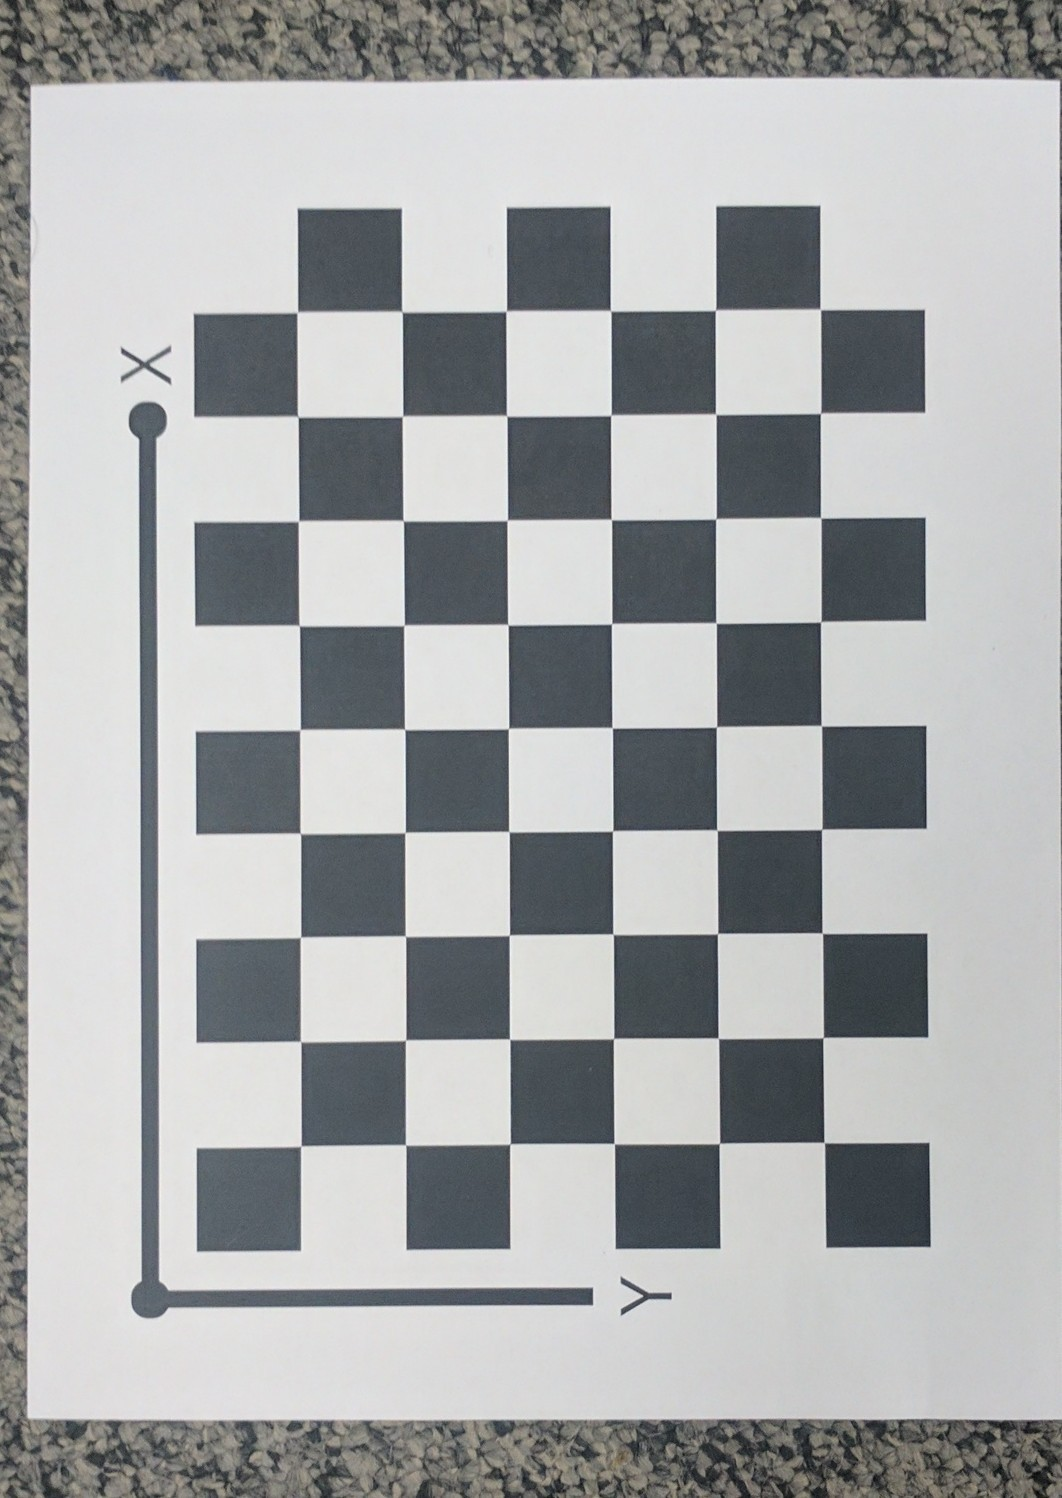
\includegraphics[scale = 0.15]{1.jpg}
%\caption{Simulation results for the network.}
\label{fig_sim}
\end{figure}

The first step is to find the pixel coordinates of the chessboard corners in each image. Points are found using the \textit{cv2.findChessboardCorners} function. The patternsize parameter is (9,6) which is the number of inner corners that are to be detected. A total of 54 corner points are found for each image.\\

Next, I specified a 3D coordinate system for each of the  54 detected points. In the 3D coordinate system the Z value is 0 for the plane of the chessboard. X and Y coordinates vary by the size of the chessboard square which is given to be 21.5 mm. The 3D coordinate system is as follows:
\begin{align*}
[0, 0, 0], [21.5, 0, 0], ... [172, 0, 0],  \\
[0, 21.5, 0], [21.5, 21.5, 0], ... [172, 21.5, 0],\\
.\\
.\\
.\\
[0, 107.5, 0], [21.5, 107.5, 0], ... [172, 107.5, 0]
\end{align*}

Now, the correspondence between the 3D coordinates and the 2D pixel coordinates are available. Next is to find the homography matrix between the 3D and 2D corresponding points. This is done with the method of direct linear transform. \\

Given n corresponding points, each corresponding pair can be used to create a 2x9 matrix as represented below:

\begin{figure}[H]
\centering
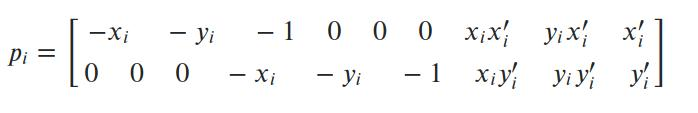
\includegraphics[scale = 0.35]{2.jpg}
%\caption{Simulation results for the network.}
\label{fig_sim}
\end{figure}

Multiple such matrices are stacked to create a matrix P. Then the system $PH = 0$ needs to be solved for H. The system is shown below:

\begin{figure}[H]
\centering
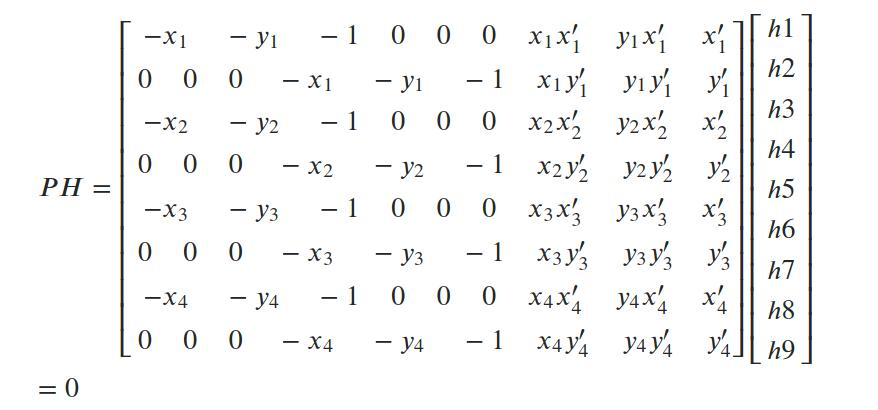
\includegraphics[scale = 0.35]{3.jpg}
%\caption{Simulation results for the network.}
\label{fig_sim}
\end{figure}

Singular value decomposition (SVD) of P is done i.e $P = USV^T$. The  last singular vector of V as the solution to H.\\

Once the Homography matrix is obtained, the matrix V which is in the closed form solution  is updated as follows:

\begin{figure}[H]
\centering
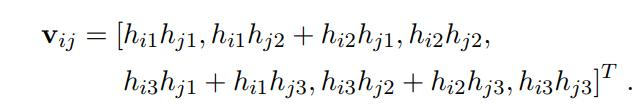
\includegraphics[scale = 0.35]{4.jpg}
%\caption{Simulation results for the network.}
\label{fig_sim}
\end{figure}

where ith column of the homography matrix is $h_i = [h_{i1}, h_{i2}, h_{i3}]^T$\\

The system can be represented as 2 homogeneous equations in b as follows:
\begin{figure}[H]
\centering
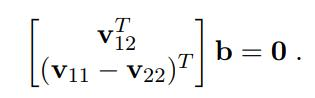
\includegraphics[scale = 0.35]{5.jpg}
%\caption{Simulation results for the network.}
\label{fig_sim}
\end{figure}

For n images, stacking n such equations, we get the system $Vb = 0$. This system is solved for b by taking SVD of V matrix and obtaining the right singular vector associated with smallest single value. Once b is obtained, it is essentially the vector $$b = [B11, B12, B22, B13, B23, B33]^T$$

This is used to solve for the intrinsic parameters of the camera matrix using the below equations:
\begin{figure}[H]
\centering
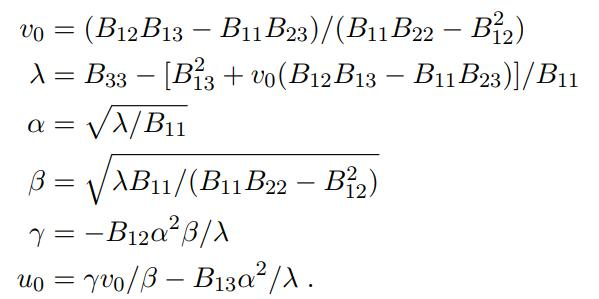
\includegraphics[scale = 0.35]{6.jpg}
%\caption{Simulation results for the network.}
\label{fig_sim}
\end{figure}

Then, the intrinsic parameter matrix is basically given by:
\begin{figure}[H]
\centering
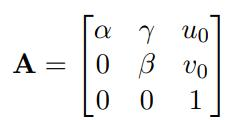
\includegraphics[scale = 0.35]{7.jpg}
%\caption{Simulation results for the network.}
\label{fig_sim}
\end{figure}

The output obtained for the above is shown below:
\begin{figure}[H]
\centering
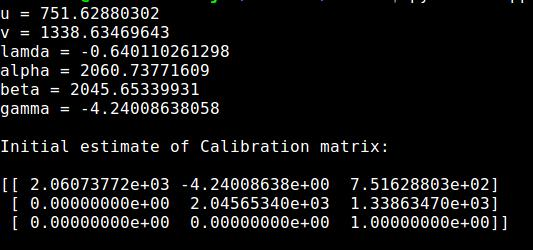
\includegraphics[scale = 0.45]{8.jpg}
%\caption{Simulation results for the network.}
\label{fig_sim}
\end{figure}

As it can be seen here, the principal point obtained is $$(u_0, v_0) = (751.6288, 1338.6347) mm$$ and focal lengths $$(f_x, f_y) = (2060.7377, 2045.653) mm $$ and skew factor is $-4.2$\\

The rotation matrix R and translation vector t for each image can be obtained from the Intrinsic matrix an = d homography matrix of that image by using the following system. \begin{figure}[H]
\centering
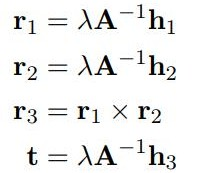
\includegraphics[scale = 0.35]{9.jpg}
%\caption{Simulation results for the network.}
\label{fig_sim}
\end{figure}

with $\lambda = 1/ \norm{A^{-1}h_1} = 1/ \norm{A^{-1}h_2}$ 

$$ R = [r_1, r_2, r_3]$$

The initial distortion is assumed to be zero and therefore $$k_c = [0,0]^T$$

\section{Non-linear Geometric Error Minimization}

First, I calculate the re-projection error before optimizing the Intrinsic parameter matrix. For each pixel coordinate in each image the error is calculated as follows:
\begin{figure}[H]
\centering
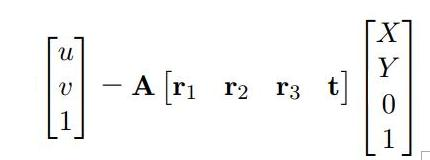
\includegraphics[scale = 0.35]{10.jpg}
%\caption{Simulation results for the network.}
\label{fig_sim}
\end{figure}

where (u, v) is the detected corner pixel coordinate, A in intrinsic matrix, [R | t] is the transformation matrix and X, Y are 3D coordinate points corresponding to the pixel coords. The error is obtained by taking the l2 norm of the resulting vector. The above process is the same as executing the following functional over all points and all images.
\begin{figure}[H]
\centering
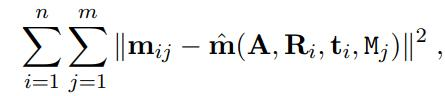
\includegraphics[scale = 0.35]{11.jpg}
%\caption{Simulation results for the network.}
\label{fig_sim}
\end{figure}

The above functional denotes the maximal likelihood estimate which assumes that the image points are corrupted by independent and identically distributed noise.  \\

The errors over all points and images is summed up and the total error is divided by (54*11) to get the mean reprojection error. The mean reprojection error before optimization is obtained as \textbf{1.24961151844} \\

To reduce the error, the functional needs to be minimized for the error while dealing with radial distortion as well. In order to obtain error due to distortion as well, the following variables are calculated:
\begin{figure}[H]
\centering
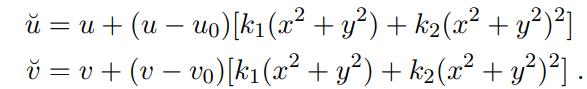
\includegraphics[scale = 0.35]{12.jpg}
%\caption{Simulation results for the network.}
\label{fig_sim}
\end{figure}


where k1 and k2 are radial distortion coefficients. $(u_0, v_0)$ is the principal point obtained from intrinsic params. $(x, y)$ is obtained from multiplying the transformation matrix with the 3D coordinates i.e
\begin{gather}
 \begin{bmatrix} x \\ y \\ 1\end{bmatrix}
 =
 [R | t]
  \begin{bmatrix}
    X \\ Y \\ 0 \\ 1
   \end{bmatrix}
\end{gather}

where R and t are rotation and translation matrix for that image.

and $(u, v)$ is obtained as 
\begin{gather}
 \begin{bmatrix} u \\ v \\ 1\end{bmatrix}
 =
 A
  \begin{bmatrix}
    x \\ y \\ 1 
   \end{bmatrix}
\end{gather}

where A is the intrinsic parameter matrix. \\

The error vector is then calculated as follows:
\begin{gather}
 \begin{bmatrix} x_p \\ y_p \end{bmatrix} -
  \begin{bmatrix}
    \widetilde{u} \\ \widetilde{v}
   \end{bmatrix}
\end{gather}


where $(x_p, y_p)$ are the pixel coordinates obtained initially thru \textit{cv2.findChessboardCorners}. The error is obtained by taking the l2 norm of the above resultant vector. \\

As previously done, the mean reprojection error is calculated take the summation over all points in all images the total summation is divided by (54*11). This error is what is to be minimized. This is done in python with the help of \textbf{scipy.optimize.least\_squares} with the cost function returning the mean reprojection error taking the radial distortion coeffs into consideration. \\

Only the intrinsic params and radial distortion coeffs are considered to minimize the error. Once the error is minimized, the result is shown as follows:
\begin{figure}[H]
\centering
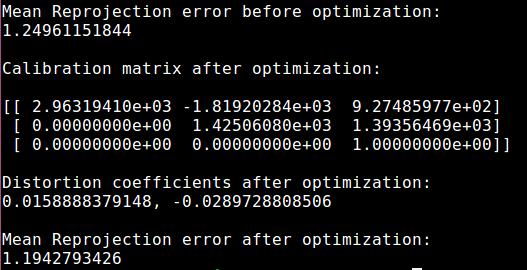
\includegraphics[scale = 0.45]{13.jpg}
%\caption{Simulation results for the network.}
\label{fig_sim}
\end{figure}
 
After optimization, the principal point obtained is $$(u_0, v_0) = (927.486, 1393.5647) mm$$ and focal lengths $$(f_x, f_y) = (2963.1941, 1425.0608) mm $$ and skew factor is $-1.8192$\\

The distortion coeffs after optimization are $$(k_1, k_2) = (0.0158888379148, -0.0289728808506)$$

The mean reprojection error after optimization is \textbf{1.1942793426}\\

The reprojected points and the original detected corners are plotted on the original images as shown below. The original detected corners are represented by blue circles and the reprojected points are denoted by red squares.

\begin{figure}[H]
\centering
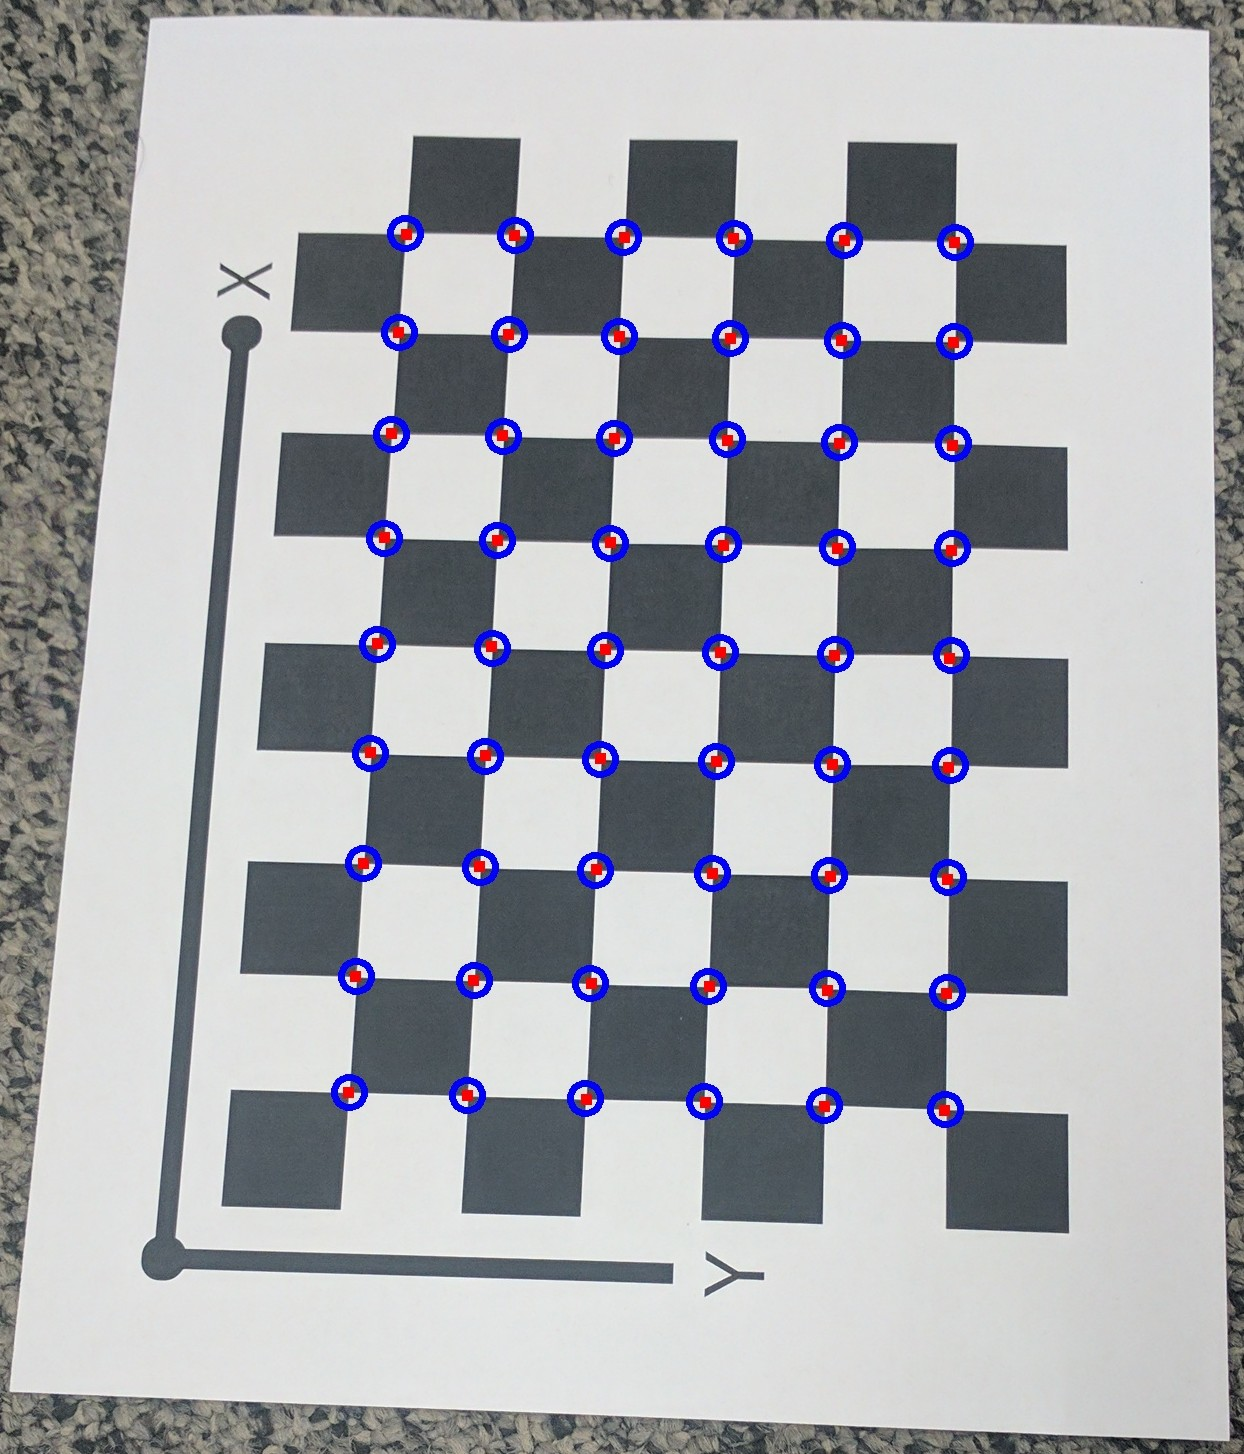
\includegraphics[scale = 0.2]{14.jpg}
%\caption{Simulation results for the network.}
\label{fig_sim}
\end{figure}

\begin{figure}[H]
\centering
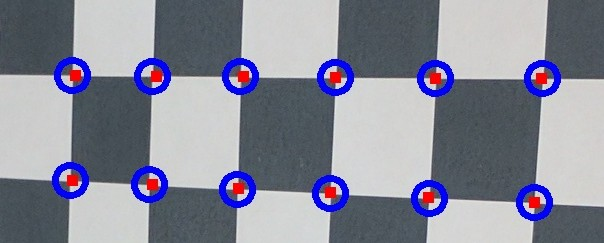
\includegraphics[scale = 0.45]{15.jpg}
%\caption{Simulation results for the network.}
\label{fig_sim}
\end{figure}

The rest of the output images are in a folder named \textit{Output} in the submission directory after running the code.




% An example of a floating figure using the graphicx package.
% Note that \label must occur AFTER (or within) \caption.
% For figures, \caption should occur after the \includegraphics.
% Note that IEEEtran v1.7 and later has special internal code that
% is designed to preserve the operation of \label within \caption
% even when the captionsoff option is in effect. However, because
% of issues like this, it may be the safest practice to put all your
% \label just after \caption rather than within \caption{}.
%
% Reminder: the "draftcls" or "draftclsnofoot", not "draft", class
% option should be used if it is desired that the figures are to be
% displayed while in draft mode.
%
%\begin{figure}[!t]
%\centering
%\includegraphics[width=2.5in]{myfigure}
% where an .eps filename suffix will be assumed under latex, 
% and a .pdf suffix will be assumed for pdflatex; or what has been declared
% via \DeclareGraphicsExtensions.
%\caption{Simulation results for the network.}
%\label{fig_sim}
%\end{figure}

% Note that the IEEE typically puts floats only at the top, even when this
% results in a large percentage of a column being occupied by floats.


% An example of a double column floating figure using two subfigures.
% (The subfig.sty package must be loaded for this to work.)
% The subfigure \label commands are set within each subfloat command,
% and the \label for the overall figure must come after \caption.
% \hfil is used as a separator to get equal spacing.
% Watch out that the combined width of all the subfigures on a 
% line do not exceed the text width or a line break will occur.
%
%\begin{figure*}[!t]
%\centering
%\subfloat[Case I]{\includegraphics[width=2.5in]{box}%
%\label{fig_first_case}}
%\hfil
%\subfloat[Case II]{\includegraphics[width=2.5in]{box}%
%\label{fig_second_case}}
%\caption{Simulation results for the network.}
%\label{fig_sim}
%\end{figure*}
%
% Note that often IEEE papers with subfigures do not employ subfigure
% captions (using the optional argument to \subfloat[]), but instead will
% reference/describe all of them (a), (b), etc., within the main caption.
% Be aware that for subfig.sty to generate the (a), (b), etc., subfigure
% labels, the optional argument to \subfloat must be present. If a
% subcaption is not desired, just leave its contents blank,
% e.g., \subfloat[].


% An example of a floating table. Note that, for IEEE style tables, the
% \caption command should come BEFORE the table and, given that table
% captions serve much like titles, are usually capitalized except for words
% such as a, an, and, as, at, but, by, for, in, nor, of, on, or, the, to
% and up, which are usually not capitalized unless they are the first or
% last word of the caption. Table text will default to \footnotesize as
% the IEEE normally uses this smaller font for tables.
% The \label must come after \caption as always.
%
%\begin{table}[!t]
%% increase table row spacing, adjust to taste
%\renewcommand{\arraystretch}{1.3}
% if using array.sty, it might be a good idea to tweak the value of
% \extrarowheight as needed to properly center the text within the cells
%\caption{An Example of a Table}
%\label{table_example}
%\centering
%% Some packages, such as MDW tools, offer better commands for making tables
%% than the plain LaTeX2e tabular which is used here.
%\begin{tabular}{|c||c|}
%\hline
%One & Two\\
%\hline
%Three & Four\\
%\hline
%\end{tabular}
%\end{table}


% Note that the IEEE does not put floats in the very first column
% - or typically anywhere on the first page for that matter. Also,
% in-text middle ("here") positioning is typically not used, but it
% is allowed and encouraged for Computer Society conferences (but
% not Computer Society journals). Most IEEE journals/conferences use
% top floats exclusively. 
% Note that, LaTeX2e, unlike IEEE journals/conferences, places
% footnotes above bottom floats. This can be corrected via the
% \fnbelowfloat command of the stfloats package.


% trigger a \newpage just before the given reference
% number - used to balance the columns on the last page
% adjust value as needed - may need to be readjusted if
% the document is modified later
%\IEEEtriggeratref{8}
% The "triggered" command can be changed if desired:
%\IEEEtriggercmd{\enlargethispage{-5in}}

% references section

% can use a bibliography generated by BibTeX as a .bbl file
% BibTeX documentation can be easily obtained at:
% http://mirror.ctan.org/biblio/bibtex/contrib/doc/
% The IEEEtran BibTeX style support page is at:
% http://www.michaelshell.org/tex/ieeetran/bibtex/
%\bibliographystyle{IEEEtran}
% argument is your BibTeX string definitions and bibliography database(s)
%\bibliography{IEEEabrv,../bib/paper}
%
% <OR> manually copy in the resultant .bbl file
% set second argument of \begin to the number of references
% (used to reserve space for the reference number labels box)
\begin{thebibliography}{1}

\bibitem{IEEEhowto:kopka}
Zhengyou Zhang, \emph{A Flexible New Technique for Camera
Calibration},  Microsoft Research, Redmond, WA, 1998.

\end{thebibliography}




% that's all folks
\end{document}


